\chapter{Ergebnisse}\label{ch:results}


\section{Ergebnisse der Basis-Modelle}\label{sec:results_basemodels}

\begin{figure}[h]
    \centering
    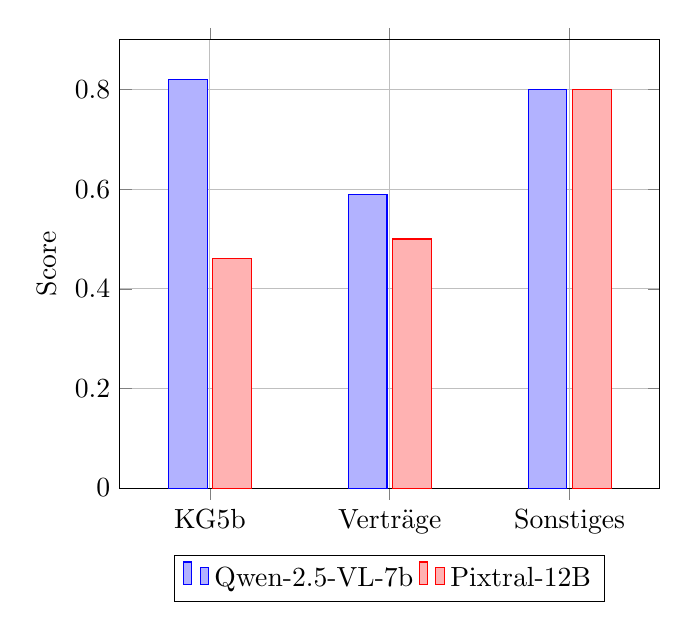
\begin{tikzpicture}
        \begin{axis}[
            ybar,
            bar width=14pt,
            ymin=0,
            ymax=0.9,
            ylabel={Score},
            symbolic x coords={KG5b, Verträge, Sonstiges},
            xtick=data,
            enlarge x limits=0.25,
            legend style={
                at={(0.5,-0.15)},
                anchor=north,
                legend columns=2
            },
            grid=major
        ]

            \addplot coordinates {
                (KG5b,0.82)
                (Verträge,0.59)
                (Sonstiges,0.80)
            };

            \addplot coordinates {
                (KG5b,0.46)
                (Verträge,0.50)
                (Sonstiges,0.80)
            };

            \legend{Qwen-2.5-VL-7b, Pixtral-12B}
        \end{axis}
    \end{tikzpicture}
    \caption{Vergleich der Modellleistungen nach Dokumentenart}
    \label{fig:result_basemodels}
\end{figure}

\section{Ergebnisse des Fine-Tunings}\label{sec:results_fine_tuning}

\section{Ergebnisse YOLO/OCR-Pipeline}\label{sec:results_yolo_ocr_pipeline}

\section{Ergebnisse im Überblick}\label{sec:results_overview}


